\documentclass[svgnames,oneside,openright,a4paper]{book}
\usepackage{tikz,booktabs}
\usepackage[danish]{babel}
\usepackage[lf]{venturis}
\usepackage[explicit]{titlesec}
\usepackage[sort&compress]{natbib}
\renewcommand*\familydefault{\sfdefault}
\usepackage[T1]{fontenc}
\usepackage[applemac]{inputenc}
\usepackage[colorlinks]{hyperref}
\usepackage{graphicx}
\bibliographystyle{astron}
\usepackage{fancyhdr}
\usepackage{varioref}
\usepackage[draft,inline]{fixme}
\usepackage{appendix}
\usepackage{amsmath,amssymb, latexsym}
\usepackage[notref,notcite,draft]{showkeys}
\usepackage[a4paper]{geometry}
\usepackage{multirow}
\parindent 0pt

% ------------------------ Header setup  ------------------------ %
\newcommand{\fncyfront}{%
	\fancyhead [RO] {{\footnotesize \rightmark}}
	\fancyfoot [RO] {\thepage}
	\fancyhead [LE] {{\footnotesize \leftmark}}
	\fancyfoot [LE] {\thepage}
	\fancyhead [RE,LO] {}
	\fancyfoot [C] {}
	\renewcommand{\headrulewidth}{0.3pt}}	
\newcommand{\fncymain}{%
	\fancyhead [RO] {{\footnotesize \rightmark}}
	\fancyfoot [RO] {\thepage} 
	\fancyhead [LE] {{\footnotesize \leftmark}}
	\fancyfoot [LE] {\thepage}
	\fancyfoot [C] {}
	\renewcommand{\headrulewidth}{0.3pt}}		
\newcommand{\fncyappendix}{%
	\fancyhead [RO] {{\footnotesize \rightmark}}
	\fancyfoot [RO] {\thepage}
	\fancyhead [LE] {{\footnotesize \leftmark}}
	\fancyfoot [LE] {\thepage}
	\fancyhead [RE,LO] {}
	\fancyfoot [C] {}	
	\renewcommand{\headrulewidth}{0.3pt}
	\renewcommand{\footrulewidth}{0.3pt}}
\makeatletter
\def\cleardoublepage{\clearpage\if@twoside
\ifodd\c@page
\else\hbox{}\thispagestyle{empty}\newpage
\if@twocolumn\hbox{}\newpage\fi\fi\fi}
\makeatother 
\pagestyle{fancy}

\include{bibliografi/abbrivations}

% ------------------------ Abstract setup  ------------------------ %
\newenvironment{abstract}%
{\cleardoublepage\null \vfill\begin{center}%
\bfseries \abstractname \end{center}}%
	{\vfill\null}

% ------------------------ Chapter setup  ------------------------ %
\newcommand*\chapterlabel{}
\titleformat{\chapter}
	{\gdef\chapterlabel{}
	  \normalfont\sffamily\Huge\bfseries\scshape}
	{\gdef\chapterlabel{\thechapter\ }}{0pt}
	{\begin{tikzpicture}[remember picture, overlay]
		\node[yshift=-4cm] at (current page.north west)
			{\begin{tikzpicture} [remember picture, overlay]
				\draw[fill=MGB] (0,0) rectangle (\paperwidth, 3cm);
				\node[anchor=west, xshift=.1\paperwidth,rectangle, rounded corners=20pt, inner sep=11pt, fill=MGR]
				{\color{white}\chapterlabel#1};
			\end{tikzpicture}
			};
		\end{tikzpicture}
	}
	\titlespacing*{\chapter}{0pt}{50pt}{-60pt}
	
% ------------------------ Custom setup  ------------------------ %	
\newcommand{\figref}[1]{figure \ref{fig:#1}}
\newcommand{\tblref}[1]{table \ref{tbl:#1}}
\newcommand{\secref}[1]{section \ref{sec:#1}}
\newcommand{\appref}[1]{appendix \ref{app:#1}}
\renewcommand{\eqref}[1]{equation (\ref{eq:#1})}
\newcommand{\chapref}[1]{chapter \ref{ch:#1}}
\graphicspath{{figures/}}	

\begin{document}
	%\raggedbottom
	\fncyfront
	\frontmatter
	\input{chapters/frontmatter}
	\input{chapters/forord}
	\tableofcontents
	\listoftables
	\listoffigures

\mainmatter
% ------------------------ Mainmatter setup  ------------------------ %	
%	- Introduktion								 %
%	- Problemformulering						 %
%	- Main									 %
%	- Konklusion								 %
% -------------------------------------------------------------------------- %

\chapter{Introduktion}
\label{ch:Intro}

Denne opgave tager sit udspring i et forl�b om verdensbilleder. Forl�bet verdensbilleder er det f�rste kernestof omr�de i l�rerplanen for alle niveauer i fysik. Denne opgaves forl�b er tilrettet l�rerplanen for fysik B \citet{FysB}. Forl�bet er essentielt da det s�tter faget ind i en historisk kontekst som mange elever finder utrolig sp�ndende. Jeg har oplevet at flere undervisere som ikke finder den videnskabshistoriske del af fysikken lige s� vigtig som de �vrige kernestof omr�der, jeg derimod har med dette forl�b valgt at fokusere s�rligt meget p� elevernes forst�else af fagets udvikling gennem tiden. Dette giver eleverne en god for-forst�else for det efterf�lgende stof. Endvidere m� vigtigheden af kendskab til videnskabshistorie understreges, hvilket bl.a. g�res af \citet{Kragh:2004}.
Forl�bet har v�ret gennemf�rt  i to naturvidenskabelige klasser p� Marselisborg Gymnasium (MARS) uafh�ngigt af hinanden. 

\section{~Naturvidenskabelige studieretninger p� MARS}
\label{sec:NVst}

Den ene klasse var 2. bm som er en klasse med bioteknologi som studieretning. Det betyder at klassen har bioteknologi A, matematik A og fysik B. Fysik forl�bet for klassen starter i 2. g. Klassen er pr�get af at denne studieretning tiltr�kker forholdsvist mange piger. 2. bm er optaget i 2011, som det fremg�r af \tblref{dreng:pige}, og markeret med r�d. Den anden klasse som har v�ret m�l for dette forl�b er 1.m som ligeledes er fremh�vet med r�d i \tblref{dreng:pige} denne studieretning tiltr�kker flest drenge. 

\begin{table}[h!]
	\centering
	\caption[K�nsfordeling p� studieretninger]{Tabellen viser k�nsfordelingen p� MARS's naturvidenskabelige studieretninger for �rene 2010/11 - 2012/13, med r�dt er markeret de klasser som har gennemf�rt forl�bet om verdensbilleder.}
	\label{tbl:dreng:pige}
	\begin{tabular}{@{ } l l l l l l l @{ }}
		\toprule[2pt]
		Optagelses	& \multicolumn{2}{c}{Biotek. (bm)}	& \multicolumn{2}{c}{Ma. - Bi. (mb)}	& \multicolumn{2}{c}{Ma. - Fy.- Ke. (m)}\\
		�r			& Piger	& Drenge				& Piger	& Drenge 				& Piger	& Drenge \\
		\midrule[1.2pt]
		2010/11		& 16		& 11					& 13		& 15					& 9		& 16\\
		2011/12		& {\color{red}21}		& {\color{red}9}					& 13		& 15					& 7		& 21\\
		2012/13		&12		& 10					& 7		& 22					& {\color{red}8}		& {\color{red}20}\\
		\bottomrule[2pt]
	\end{tabular}
\end{table}

\begin{figure}[h!]
	\centering
	\includegraphics[width=.4\textwidth,angle=-90]{optag}
	\caption[Elevoptag p� naturvidenskabelige studieretninger]{Optag af hhv. drenge og piger p� naturvidenskabelige studieretninger inden for de sidste tre �r p� Marselisborg Gymnasium}
	\label{fig:optag}
\end{figure}

P� \figref{optag} ser vi at antallet af optagne piger i bm-klassen svarer nogenlunde til optaget af drenge i m-klassen. Dette er dog ikke g�ldende for klasser optaget i august 2012. Her ses en klar overv�gt af drenge i b�de mb-klassen og i m-klassen, mens bm-klassen er mere j�vnt fordelt p� k�n. Herunder f�lger en beskrivelse af de to klasser hvori forl�bet har v�ret k�rt. Det drejer sig om nuv�rende 2.bm og nuv�rende 1.m grunden til at de to klasser er valgt er at de begge har gennemg�et forl�bet om verdensbilleder samt at de er to vidt forskellige steder i deres gymnasiale forl�b og dermed er deres kognitive niveau ogs� vidt forskelligt. 

\subsection{~bm optaget august 2011}
\label{sub:2bm}
Klassen 2.bm er en klasse der er meget domineret af det store antal piger i klassen. Klassen har en naturlig naturvidenskablig interesse som g�r i den biologiske retning hvilket ogs� afspejles i klassens valg af stuideretningsfag. Klassen har det dog generelt lidt sv�rer med de tunge naturvidenskabelige decipliner s� som fysik. Dette skyldes at de har det sv�rt ved den underliggende matematik. 2.bm er pr�get meget af at der er mange elever som har det sv�rt psykisk, og at der er en del gruppe dannelse. Hvilket medvirker til at eleverne let frustreres over faglige udfordringer og at klassen let falder i f�lden med at snakke om weekenden frem for at arbejde med det stof som forel�gges klassen. Fokus for denne klasse med forl�bet har v�ret at lave s�rligt elevaktiverende undervisning. For at s�tte eleverne i centrum for undervisningen og for at skabe en forundring over det verdensbillede vi har idag, og dets opst�en. 

\subsection{~m optaget august 2012}
\label{sub:1m}
Klassen 1.m er pr�get af en stor overv�gt af drenge. K�nsfordelingen i klassen er omvendt af af den fordeling der er i klassen 2.bm. Klassen 1.m er en ABB studieretning med matematik p� A niveau og fysik og kemi p� B niveau. I denne klasse har eleverne rigtig godt fat i matematikken og dermed rigitg gode foruds�tninger for at arbejde med fysik. Eleverne er meget sp�rgelystne og er naturligt meget nysgerrige, hvilket er godt for den faglige udvikling. Forl�bet blev oprindeligt gennemf�rt i 2.bm og efterf�lgende tilpasset til 1.m baseret p� de kommentarer der blev givet i hhv. den mundtlige og den skriftlige evaluering af forl�bet. Forl�bets fokus i 1.m har v�ret, arbejdet i grupper samt skabe en faglig erkendelse som skaber den n�dvendige indsigt for den videre progression i faget fysik.

\section[JTI/MBTI]{~2 klasser ca. 60 elever og 16 personligheder}
\label{sec:2kl}
Vi har som beskrivet i \secref{NVst} har vi 2 klasser som udgangspunkt for denne opgave dermed har vi godt og vel 60 elever. Det betyder at vi har 60 forskellige personligheder som skal have stoffet serveret p� hver deres m�de. Derfor er det n�dvendigt at vide noget om hvorledes forskellige typer at personligheder skal have viden serveret for at f� det optimale ud af undervisningen. Derfor er det af vital betydning for den enkelte underviser at have kendskab til f.eks. Jungs personligheds teorier \citep{jung1923psychological,JTI, Ringstad:2002}. Disse er sammen med videre udviklingen ved Myers og Briggs \citep{MBTI} blevet til at en personlighed sammens�ttes af fire pr�ferencer disse v�lges udfra nedenst�ende mods�tningspar. For en uddybende forklaring af betydningen af hver enkelt pr�ference kan \citet{Ringstad:2002} konsulteres.
\begin{center}
	\begin{tikzpicture}
		%\draw[thin, draw=LightSkyBlue, anchor=south west, step=1mm] (0,0) grid (10,10);
		%\draw[draw=blue,anchor=south west, step=5mm] (0,0) grid (10,10);
		%\draw[thick,draw=SkyBlue,anchor=south west, step=10mm] (0,0) grid (10,10);
		
		\draw[thin, black] (2,5.5) -- (8,5.5) -- (8,8) -- (2,8) -- cycle;
		\draw[thick, black] (4.7,7.7) -- (5.3,7.7);
		\draw[thick, black] (4.7,7.2) -- (5.3,7.2);
		\draw[thick, black] (4.7,6.7) -- (5.3,6.7);
		\draw[thick, black] (4.7,6.2) -- (5.3,6.2);
		
		\node[black,left] at (4.5,7.6) {Ekstrovert ({\bf E})};
		\node[black,left] at (4.5,7.2) {Sansning ({\bf S})};
		\node[black,left] at (4.5,6.7) {T�nkning ({\bf T})};
		\node[black,left] at (4.5,6.2) {Judging ({\bf J})};
		
		\node[black,right] at (5.5,7.6) {({\bf I}) Introvert};
		\node[black,right] at (5.5,7.2) {({\bf N}) INtuition};
		\node[black,right] at (5.5,6.7) {({\bf F}) F�lelse};
		\node[black,right] at (5.5,6.2) {({\bf P}) Perseption};
	\end{tikzpicture}
\end{center}

Med afs�t i denne tankegang kaldet Jungian Type Indicator (JTI) eller Myers-Briggs Type Indicator (MBTI) kan vi sammens�tte 16 forskellige personligheder. Disse fremg�r af \figref{MBTI} herunder.  P� baggrund af personlighederne i nedenst�ende skema kan vi ved hj�lp af de to midterste bogstaver i hvert personlighed definere nogle f�llestr�k dette betyder at vi f�r nogle r�de personligheder (sanse - t�nke) typer, nogle gule (sanse - f�le) typer, nogle gr�nne (intuition - f�le) typer og nogle bl� (intuition - t�nke) typer, alle beskrevet i stor detalje i \citet{Alstrup:1997,DDS:2006}.
\begin{figure}[h!]
	\centering
	\begin{tikzpicture}
		%\draw[thin, draw=LightSkyBlue, anchor=south west, step=1mm] (0,0) grid (10,10);
		%\draw[draw=blue,anchor=south west, step=5mm] (0,0) grid (10,10);
		%\draw[thick,draw=SkyBlue,anchor=south west, step=10mm] (0,0) grid (10,10);
		%
		%% DEFINE COLORS
		\definecolor{r1}{cmyk}{0.08,0.36,0.21,0}
		\definecolor{y1}{cmyk}{0.02,0.21,0.33,0}
		\definecolor{g1}{cmyk}{0.2,0.04,0.36,0}
		\definecolor{b1}{cmyk}{0.33,0.14,0.01,0}
		
		%% DEFINE COLORED REGIONS
		\draw[very thin, fill=r1] (1,1) -- (3,1) -- (3,9) -- (1,9) -- cycle;
		\draw[very thin, fill=y1] (3,1) -- (5,1) -- (5,9) -- (3,9) -- cycle;
		\draw[very thin, fill=g1] (5,1) -- (7,1) -- (7,9) -- (5,9) -- cycle;
		\draw[very thin, fill=b1] (7,1) -- (9,1) -- (9,9) -- (7,9) -- cycle;
		
		%% DRAW THE VERTICAL GRID
		\draw[very thick, black] (1,9) -- (9,9);
		\draw[very thick, black] (1,7) -- (9,7);
		\draw[very thick, black] (1,5) -- (9,5);
		\draw[very thick, black] (1,3) -- (9,3);
		\draw[very thick, black] (1,1) -- (9,1);
		
		%% DRAW THE HORIZONTAL GRID
		\draw[very thick, black] (9,1) -- (9,9);
		\draw[very thick, black] (7,1) -- (7,9);
		\draw[very thick, black] (5,1) -- (5,9);
		\draw[very thick, black] (3,1) -- (3,9);
		\draw[very thick, black] (1,1) -- (1,9);
		
		%% TOP LETTERS
		\node[black] at (2,9.5) {\fontspec[SizeFeatures={{Size=14}}]{Neo Tech Std}S};
		\node[black] at (4,9.5) {\fontspec[SizeFeatures={{Size=14}}]{Neo Tech Std}S};
		\node[black] at (6,9.5) {\fontspec[SizeFeatures={{Size=14}}]{Neo Tech Std}N};
		\node[black] at (8,9.5) {\fontspec[SizeFeatures={{Size=14}}]{Neo Tech Std}N};
		
		
		%% LEFT SIDE LETTERS
		\node[black] at (0.5,8) {\fontspec[SizeFeatures={{Size=14}}]{Neo Tech Std}I};
		\node[black] at (0.5,6) {\fontspec[SizeFeatures={{Size=14}}]{Neo Tech Std}I};
		\node[black] at (0.5,4) {\fontspec[SizeFeatures={{Size=14}}]{Neo Tech Std}E};
		\node[black] at (0.5,2) {\fontspec[SizeFeatures={{Size=14}}]{Neo Tech Std}E};
		
		%% RIGHT SIDE LETTERS
		\node[black] at (9.5,8) {\fontspec[SizeFeatures={{Size=14}}]{Neo Tech Std}J};
		\node[black] at (9.5,6) {\fontspec[SizeFeatures={{Size=14}}]{Neo Tech Std}P};
		\node[black] at (9.5,4) {\fontspec[SizeFeatures={{Size=14}}]{Neo Tech Std}P};
		\node[black] at (9.5,2) {\fontspec[SizeFeatures={{Size=14}}]{Neo Tech Std}J};
		
		%% BOTTOM LETTERS
		\node[black] at (2,.5) {\fontspec[SizeFeatures={{Size=14}}]{Neo Tech Std}T};
		\node[black] at (4,.5) {\fontspec[SizeFeatures={{Size=14}}]{Neo Tech Std}F};
		\node[black] at (6,.5) {\fontspec[SizeFeatures={{Size=14}}]{Neo Tech Std}F};
		\node[black] at (8,.5) {\fontspec[SizeFeatures={{Size=14}}]{Neo Tech Std}T};
		
		%% TYPE INDICATORS
		\node[black] at (2,8) {\fontspec[SizeFeatures={{Size=14}}]{Neo Tech Std}ISTJ};
		\node[black] at (2,6) {\fontspec[SizeFeatures={{Size=14}}]{Neo Tech Std}ISTP};
		\node[black] at (2,4) {\fontspec[SizeFeatures={{Size=14}}]{Neo Tech Std}ESTP};
		\node[black] at (2,2) {\fontspec[SizeFeatures={{Size=14}}]{Neo Tech Std}ESTJ};
		
		\node[black] at (4,8) {\fontspec[SizeFeatures={{Size=14}}]{Neo Tech Std}ISFJ};
		\node[black] at (4,6) {\fontspec[SizeFeatures={{Size=14}}]{Neo Tech Std}ISFP};
		\node[black] at (4,4) {\fontspec[SizeFeatures={{Size=14}}]{Neo Tech Std}ESFP};
		\node[black] at (4,2) {\fontspec[SizeFeatures={{Size=14}}]{Neo Tech Std}ESFJ};
		
		\node[black] at (6,8) {\fontspec[SizeFeatures={{Size=14}}]{Neo Tech Std}INFJ};
		\node[black] at (6,6) {\fontspec[SizeFeatures={{Size=14}}]{Neo Tech Std}INFP};
		\node[black] at (6,4) {\fontspec[SizeFeatures={{Size=14}}]{Neo Tech Std}ENFP};
		\node[black] at (6,2) {\fontspec[SizeFeatures={{Size=14}}]{Neo Tech Std}ENFJ};
		
		\node[black] at (8,8) {\fontspec[SizeFeatures={{Size=14}}]{Neo Tech Std}INTJ};
		\node[black] at (8,6) {\fontspec[SizeFeatures={{Size=14}}]{Neo Tech Std}INTP};
		\node[black] at (8,4) {\fontspec[SizeFeatures={{Size=14}}]{Neo Tech Std}ENTP};
		\node[black] at (8,2) {\fontspec[SizeFeatures={{Size=14}}]{Neo Tech Std}ENTJ};
	\end{tikzpicture}
	\caption[Jungs Type Indicator]{Skematisk opstilling af de 16 mulige personligheder som tillades jf. Jungs teori, \citep{jung1923psychological,JTI, Ringstad:2002, MBTI}.}
	\label{fig:MBTI}
\end{figure}
F�lles for disse fire typer at de har nogle h�ndgribelige tr�k som man som underviser b�r v�re opm�rksom p� i sin omgang med elever, og tage h�jde for n�r man planl�gger sin undervisning, og specielt i forhold til elev aktiverende undervisning. De to tabeller herunder \tblref{DDS:seek} og \tblref{DDS:avoid} fremg�r det hvad det er for nogle tr�k man hos eleverne kan v�re opm�rksom p� der kan give en nogle hints til hvordan eleverne skal have opgaverne serveret og hvilke undervisningsformer man helst skal undg� for at fremme elevernes ind l�ring begge tabeller er hentet fra \citet{DDS:2006}, og farve angivelserne svare til dem angivet p� \figref{MBTI}.
\begin{table}[h!]
	\centering
	\caption[De fire ledertyper fra \citep{DDS:2006} s�ger]{De fire ledertyper fra \citet{DDS:2006}, baseret p� JTI/MBTI, s�ger:}
	\label{tbl:DDS:seek}
	\begin{tabular}{@{ } p{3.25cm} p{3.25cm} p{3.25cm} p{3.25cm} @{ }}
		\toprule[2pt]
			R�de			& Gule			& Gr�nne				& Bl�\\
			Sanse-/t�nketypen	& Sanse-/f�letypen	& Intuitions-/f�letypen	& \mbox{Intuitions-/}\mbox{t�nketypen}\\
		\midrule[1.25pt]
			At overv�ge gruppens udvikling ved hj�lp af budgetter, regnskaber, medlemstal osv.	&	At bruge afpr�vede og gennemt�nkte metoder	&	At fremme gl�de, harmoni og nyskabelse	&	At f� gruppen til at fokusere p� fremtiden\\
		\midrule[.5pt]
			At styre udgifter og handlingsplaner	&	At anvende sine erfaringer p� praktiske opgaver	&	At udf�rer arbejder der �bner mulighed for ny viden og udvikling	&	At k�de planer, metoder og modeller sammen\\
		\midrule[.5pt]
			At vise h�ndgribelige resultater	&	At fordele arbejdet retf�rdigt	&	At kommunikere p� kreative m�der	&	at finde muligheder for udvikling i gruppen\\
		\midrule[.5pt]
			At anvende afpr�vede metoder til at skabe succes	& At gennemg� planer og materialer som andre har udformet, for at finde frem til hvad der virker bedst	&	At skaffe sig indsigt i ting der er betydningsfulde for gruppens medlemmer	&	At unders�ge komplekse problemers langsigtede virkning\\
		\midrule[.5pt]	
			At l�se problemer med det samme	&		&	At arbejde p� mange forskellige m�der for at f� succes	&	At diskutere udfordrende sp�rgsm�l\\
		\bottomrule[2pt]
	\end{tabular}
\end{table}
\begin{table}[h!]
	\centering
	\caption[De fire ledertyper fra \citep{DDS:2006} undg�r]{De fire ledertyper fra \citet{DDS:2006}, baseret p� JTI/MBTI, undg�r:}
	\label{tbl:DDS:avoid}
	\begin{tabular}{@{ } p{3.25cm} p{3.25cm} p{3.25cm} p{3.25cm} @{ }}
		\toprule[2pt]
			R�de			& Gule			& Gr�nne				& Bl�\\
			Sanse-/t�nketypen	& Sanse-/f�letypen	& Intuitions-/f�letypen	& \mbox{Intuitions-/}\mbox{t�nketypen}\\
		\midrule[1.25pt]
			At deltage i alt for sociale ("langh�rede") aktiviteter	&	At anvende nye og upr�vede metoder	&	At tage sig af kontrolfunktioner s� som regnskaber	&	At g�re andres arbejde\\
		\midrule[.5pt]
			Brainstorm som ikke medf�rer noget praktisk resulatat	&	At diskuteres forskellige teorierns fordele	&	At opstille hierakier og kommandoveje	&	At kappes med andre om popularitet\\
		\midrule[.5pt]
			At opstille hypoteser om fremtiden	&	At analysere og forudsige resultater af strategiske planer	&	Intriger	&	At arbejde med administrative detaljer\\
		\midrule[.5pt]
			At anvende uafpr�vede og ikke gennemt�nkte metoder	&	At komme med kritik i et �bent forum, is�r i relation til gruppemedlemmer som de kender	&	At tage sig af papirnusseri	&	At udf�rer rutinearbejde\\
		\midrule[.5pt]
			Manglende koncentration om arbejdet	&	At behandle andre mennesker som "udskiftelige manskindele"	&		&	At deltage i alt for sociale ("langh�rede") aktiviteter\\
		\bottomrule[2pt]
	\end{tabular}
\end{table}

Basseret p� disse teorier vil vi typisk se at ca. halvdelen af de elever vi underviser vil optr�de Introverte med andre ord, de ``\emph{t�nker for at tale}'' mens de resterende er ekstroverte, de ``\emph{taler for at t�nke}''. Vores skolesystem er som udgangspunkt indrettet efter elever som t�r sige noget alts� de ekstroverte, da vi bel�nner eleverne med en mundtlig karakter. Derfor er det op til den enkelte underviser at sikre at de introverte ogs� f�r lejlighed til at sige noget. Derfor kan det v�re godt at lave sm� summe grupper da de introverte elever derved f�r l�ngere tid til at t�nke sig om, inden undervisningen er n�et til et nyt emne. Betragter man de to klasser 1.m og 2.bm burde man statistisk set skulle observere at eleverne fordeler sig j�vnt mellem de fire farve kategorier, fra \citet{Alstrup:1997,DDS:2006}, imidlertid viser det sig, at eleverne i de to klasser hovedsageligt er r�de og gule typer mens der er f� gr�nne og bl�, jf \figref{MBTI}. Da vi nu kender lidt til de to klasser som forl�bet har v�ret gennemf�rt i, er det naturligt at se p� problemstillingen som forholder sig til den faglige progression n�r vi arbejder med mange forskellige elev personligheder.
\chapter{V�rkt�jskassen}
\label{ch:Beg}
\epigraph{Giv mig et sted at st�, og jeg skal bev�ge verden!}{Arkimedes}


I v�rkt�jskassen er der beskrevet nogle f� essentielle v�rkt�jer, man som underviser med fordel kan anvende til at sikre den faglige progression. Der er dog anvendt v�rkt�jer som kr�ver en uddybende forklaring. Disse forklaringer er henlagt til opgavens appendix. Vi vil dog ikke gennemg� den didaktiske metode, FIMME, som vi har gennemg�et i stor detalje p� AP1, W1, se endvidere \citep[s. 275]{Gympd}. 

\section{~L�ring}
\label{sec:teach}
Med udgangspunkt i Piagets radikalkonstruktivisme og Deweys Learning by doing opfattes l�ring som David Kolbs - Erfaringsbasserede l�ring \citep{Kolb:1984,Illeris, Gympd}. Kolbs teorier tager sit udgangspunkt i bl.a. John Deweys ``Learning by doing'' \citep{Dewey:1978, Gympd} -- hvor fokus l�gges p� handlen og ageren i verden. Grundlaget for at v�lge denne l�ringsopfattelse er at den erkendelsesbasserede rationelle l�ring oftest ligger i god tr�d med den naturvidenskablige m�de at t�nke p�. Endvidere er det et udtryk for den baggrund jeg har fra spejderbev�gelsen hvor Deweys mantra ``Learning by doing'' altid har v�ret et motto. Foruden Dewey bygger kolbs teori p� andre l�ringsteoretikkere som Kurt Lewin og Jean Piaget, som alle ser l�ring som en natur sp�ndings- og konfliktfyldt aktivitet. De har hver is�r deres konflikt par. Hvor Dewey  og Lewin arbejder med mods�tningen mellem indtryk og tanker eller id�er alts� den konkrete erfaring mod de abstrakte begreber. S� arbejder Piaget med l�ringen som vekselvirkningen mellem akkommodation af id�er og assimilation af erfaring alts� en vekselvirkning mellem den aktive eksperimenteren og de reflekterende observationer. Dette giver anledning til den vandrette og den horisontale akse i Kolbs l�ringsmodel (se \figref{kolb1}), Se endvidere \tblref{Kolb} for en konkret mere information om den konkrete l�ring i f�lge Kolb.
\begin{figure}[hbt]
	\centering
	\begin{tikzpicture}
		%\draw[very thin, lightgray, step=1mm] (0,0) grid (10,10);
		%\draw[thin, gray, step=5mm] (0,0) grid (10,10);
		%\draw[thick, darkgray, step=10mm] (0,0) grid (10,10);
		
		% WRITE THE FOUR POINTS
		\node at (0,5.3) {Aktiv};
		\node at (0,5) {eksperimenteren};
		
		\node at (5,10) {konkret};
		\node at (5,9.7) {erfaring};
		
		\node at (10,5.3) {Reflekterende};
		\node at (10,5) {observation};
		
		\node at (5,.3) {Abstrakt};
		\node at (5,0) {begrebsdannelse};
		
		% PLACE ROUND ARROWS
		\draw[very thick, blue!40!white, ->, rotate=-90] (-.5,4) arc (0:-90:4cm);
		\draw[very thick, blue!40!white, ->, rotate=180] (0,-5.75) arc (0:-90:4cm);
		\draw[very thick, blue!40!white, ->, rotate=90] (9.75,-6) arc (0:-90:4cm);
		\draw[very thick, blue!40!white, ->, rotate=0] (10,4.5) arc (0:-90:4cm);

		% DRAW VERTICAL AND HORIZONTAL ARROW
		\draw[very thick, blue!80!black, <->] (5,.5) -- (5,9.5);
		\draw[very thick, blue!80!black, <->] (1.5,5) -- (9,5);
		
		% DRAW NOTES
		\node[draw=white, fill=white, text=black] at (5,2) {Begribelse via};
		\node[draw=white, fill=white, text=black] at (5,1.5) {BEGREBSBASERET REFLEKSION};
		
		\node[draw=white, fill=white, text=black] at (5,8.5) {Begribelse via};
		\node[draw=white, fill=white, text=black] at (5,8.0) {UMIDDELBAR OPLEVELSE};
		
		\node[draw=white, fill=white, text=black] at (3,5.3) {Omdannelse via};
		\node[draw=white, fill=white, text=black] at (3,4.7) {AKTIV HANDLEN};
		
		\node[draw=white, fill=white, text=black] at (7,5.3) {Omdannelse via};
		\node[draw=white, fill=white, text=black] at (7,4.7) {MENINGSTILSKRIVELSE};
		
		\node[red] at (3,7) {Akkumolativ erkendelse};
		\node[red] at (7,7) {Divergent erkendelse};
		\node[red] at (3,3) {Konvergent erkendelse};
		\node[red] at (7,3) {Assimilativ erkendelse};
	\end{tikzpicture}
	\caption[Kolbs l�ringsmodel]{Kolbs l�ringsmodel \citep[side 42]{Kolb:1984} og \citep[side 177]{Gympd}}
	\label{fig:kolb1}
\end{figure}
\begin{table}
	\centering
	\caption[Kolbs l�ringstilgange]{Kolbs L�ringstilgange \citep[side 347]{Gympd}}
	\label{tbl:Kolb}
	\begin{tabular}{l l p{6cm}}
		\toprule[2pt]
		Erkendelsesform & L�ringstilgang & Egenskaber hos den l�rende\\
		\midrule
		\multirow{4}{*}{Divergent erkendelse} 	& \multirow{2}{*}{Konkret erfaring} 			& Udviklet forestillingsevne\\ 
										&									& God til at udvikle id\'eer og unders�ge ud fra forskellige perspektiver\\
										& \multirow{2}{*}{Reflekterende observation}	& Interesserer sig for mennesker\\
										&									&  Bredt interessefelt (kulturelt) \\
		\midrule
		\multirow{3}{*}{Assimilativ erkendelse}	& Abstrakt begrebsligg�relse				& Udviklet evne til at danne teoretiske modeller\\
										& \multirow{2}{*}{Reflekterende observation}	& God til induktiiv r�sonnering\\
										&									& Interesse for abstract begreber frem for mennesker\\
		\midrule
		\multirow{4}{*}{Konvergent erkendelse}	& \multirow{2}{*}{Abstrakt begrebsligg�relse}	& St�rk i praktisk anvendelse af id\'eer\\
										&									& God til deduktivt r�sinnement\\
										& \multirow{2}{*}{Aktiv eksperimenteren}		& Ikke f�lelsesbetonet\\
										&									& Sn�vert interessefelt\\
		\midrule
		\multirow{4}{*}{Akkumulativ erkendelse}	& \multirow{2}{*}{Konkret erfaring}			& Allerbedst til at handle\\
										&									& L�ber gerne en risiko/er chancerytter\\
										& \multirow{2}{*}{Aktiv esperimenteren}		& God til at handle ``i nuet''\\
										&									& L�ser problemer intuitivt\\
		\bottomrule[2pt]
	\end{tabular}
\end{table}

Det nye i Kolbs l�ringsmodel i forhold til tidligere er at Kolb introducere en individuel erfarings tilgang til det kognitive begrebs apparat som Piaget og mentalismen st�r for. og derved bringer sociokulturalismen ind i l�ringen gennem praksisf�llesskaber, gennemg�et p� AP2 og i \citep{Wenger:2007}. 

\begin{quote}
	``\emph{L�ring er n�r sindet udfordres p� et passende kognitivt niveau s�ledes at den l�rende er i stand til at reflektere over egen l�ring}''
\end{quote}

Tager vi udgangspunkt i \figref{kolb1} kan denne illustrere hvorledes en elev er n�dt til at bearbejde et f�nomen f�r der er tale om l�ring. Eleven og underviseren skal nemlig hele vejen rundt om Kolbs l�rings cirkel for at eleven opn�r den fulde l�ring. Dette kan side stilles med 4MAT\textregistered~ modellen, gennemg�et i \appref{4MAT}, hvor man ligeledes skal helevejen rundt om hjulet, se \figref{4MAT}, inden man kan tale om fuldkommen l�ring.  4MAT\textregistered~modellen er et glimrende v�rkt�j til didaktisering af enkeltst�ende aktiviteter eller l�ngerevarende forl�b da det sikre at man som underviser for vendt vigtige aspekter af undervisningen, samtidig hj�lper den til at huske at fokusere p� de forskellige elevtyper man har i klasserummet. Dermed kan man sikre den faglige progression bedre for den enkelte elev. 

Et andet nyttigt v�rkt�j man som underviser kan anvende for at f� sin undervisning til at v�re helst�bt og god for eleverne er den didaktiske relations model, som beskrives i detalje i \appref{relation}

\section{~Faglige progression}
\label{sec:DFP}

\begin{wrapfigure}{r}{7.5cm}
	\vspace{-10pt}
	\centering
	\includegraphics[width=5cm]{kort}
	\caption{Illustration af korthuset fra \citep{Christensen:2006}}
	\label{fig:kort}
	\vspace{-10pt}
\end{wrapfigure}
N�r vi snakker om den faglige progression og de forestillinger som vi som undervisere har om progression er det naturligt at konsultere \citep{Christensen:2006, Gympd, EVA:2011, Jacobsen:2008M,Johannsen:2009M,Warson:2000}. Her er stort set alle forestillinger vi har om progressionen gennemg�et og vi vil kort ridse nogle op. En af de skematikker som fremh�ves i artiklen er i s�rdeleshed forestillingen om progression som v�rende noget der bev�ger sig fra at v�re nemt til at v�re sv�rt, eller fra noget som er konkret til noget som er mere abstrakt. Alternativt kan man snakke om mods�tningen simpel - kompleks. Denne forestilling er typisk for de naturvidenskabelige fag, og er som s�dan ogs� anvendt i dette forl�b. Denne progressions forestilling beskrives ofte ved et korthus, se \figref{kort}, analogien beskriver processen hvor underviseren med stor omhu tilrettel�gger undervisningen, laver underviseren blot en forkert bev�gelse s� braser det hele sammen. N�r vi snakker om korthuset snakker vi endvidere om processen to skridt frem og et tilbage som forholder sig til det faktum at vi hele tiden skal sikre at eleverne er med. I samme �ndedrag kunne man sige at det nytter ikke noget at bygge taget p� korthuset hvis man ikke har et fundament og et stueplan. Man bygger alts� ting op nedefra.

\begin{wrapfigure}{l}{7.5cm}
	\vspace{-10pt}
	\centering
	\includegraphics[width=5cm]{trappe}
	\caption{Illustration af trappen fra \citep{Christensen:2006}}
	\label{fig:trappe}
	\vspace{-10pt}
\end{wrapfigure}
En anden tilgang til progression er ved hj�lp af taksonomi i de kognitive niveauer som der skrives i artiklen. Dette kendes i stor detalje i den m�de STX er struktureret p� her tales ofte om Blooms taksonomi \citep{Gympd, Krathwool:2002} der kan illustreres som en  trappe jf. \figref{trappe}. Den Bloomske taksonomi egner sig dog ikke s� godt til de naturvidenskablige fag da vi har en anden betydning af de taksonomiske niveauer: viden, forst�else, anvendelse, analyse, syntese og vurdering. S� niveauer som er h�jt v�gtet i naturvidenskablige vil ikke n�dvendigvis v�re det i humanistiske fag grundet menings tilskrivelsen, der mangler en tv�r fakult�r diskurs for betydningen af de taksonomiske niveauer. Derfor er flere naturvidenskabsfolk g�et over til SOLO-taksonomien som beskrevet i \chapref{Afv} og illustreret med \figref{SOLO}.

I de naturvidenskabelige fag er underviseren i h�j grad underlagt en progression i form af l�replanen \citep{FysB} her bliver det af \citep{Christensen:2006} fremh�vet at s�rligt i matematik men ogs� i fysik lider underviserne under manglende frihed til at styre progressionen da der fra ministeriel h�nd er stram styring med det stof der skal gennemg�es. Dermed har man fra ministeriet sikret at der er en naturlig progression indlagt i forl�bet. Dertil kommer selvf�lgelig den progression som man kan l�gge ind i sin undervisning i forhold til de m�l man s�tter for eleverne i forhold til et forl�b. Som tidligere omtalt handler progression ogs� om ledelse alts� hvordan man guider eleverne videre taksonomisk dette kan ske b�de gennem sp�rgeteknik men der er ogs� mange andre m�der. Man kan hj�lpe eleverne p� vej til selv at udvide deres sp�rgehorisont jf. IBS tanken, \citep{Flick:2006,Michelsen:2011M, Meyer:2008, leder:2010, EVA:2013}

Forl�bet om verdensbilleder passer godt ind i fundamentet for korthuset Fysik B-niveau. Da man skal have en forst�else for det verdenssyn man havde tidligere den udvikling der er sket frem til idag for at man kan forholde sig til de forandringer der vil komme efterh�nden som der g�res nye opdagelser inden for naturvidenskaben. Forl�bet er alts� det fundament vi skal bygge vores forst�else af fysikken p�. Endvidere kr�ver forl�bet ikke forudg�ende kendskab til fysik og matematik for at kunne deltage hvilket g�r det ideelt til introduktionsforl�b. 

%N�r vi t�nker p� den faglige progression i forhold til eleverne med den radikal konstruktivistiske tilgang som beskrives gennem Piaget \citep{Gympd}. Har vi med unge mennesker at g�re og dermed vil vores elever typisk v�re i den formalt-operationelle periode hvilket betyder at eleverne begynder at foretage abstrakte intellektuelle operationer. Et typisk undervisnings forl�b vil tage afs�t i den viden som allerede findes blandt eleverne, dette ses i forl�bet om verdensbilleder i at man starter en hurtigskrivning. Dette tjener som en afd�kning af for-forst�elsen men ligeledes til repiterere allerede kendt stof. Efterf�lgende tilstreber man at organisere viden p� en ny m�de. Man aktivere s� at sige langtidshukommelsen og man skaber da hierarkier i den viden som eleverne har. Tilslut skaber man forbindelser mellem ny og tidligere viden  herved udvides elevernes horisont\footnote{Som fremh�vet p� slides fra AP2}. 

\section{~Teoretisk udgangspunkt for forl�bet}
\label{sec:FTU}
\begin{wrapfigure}{r}{7.5cm}
	\vspace{-10pt}
	\centering
	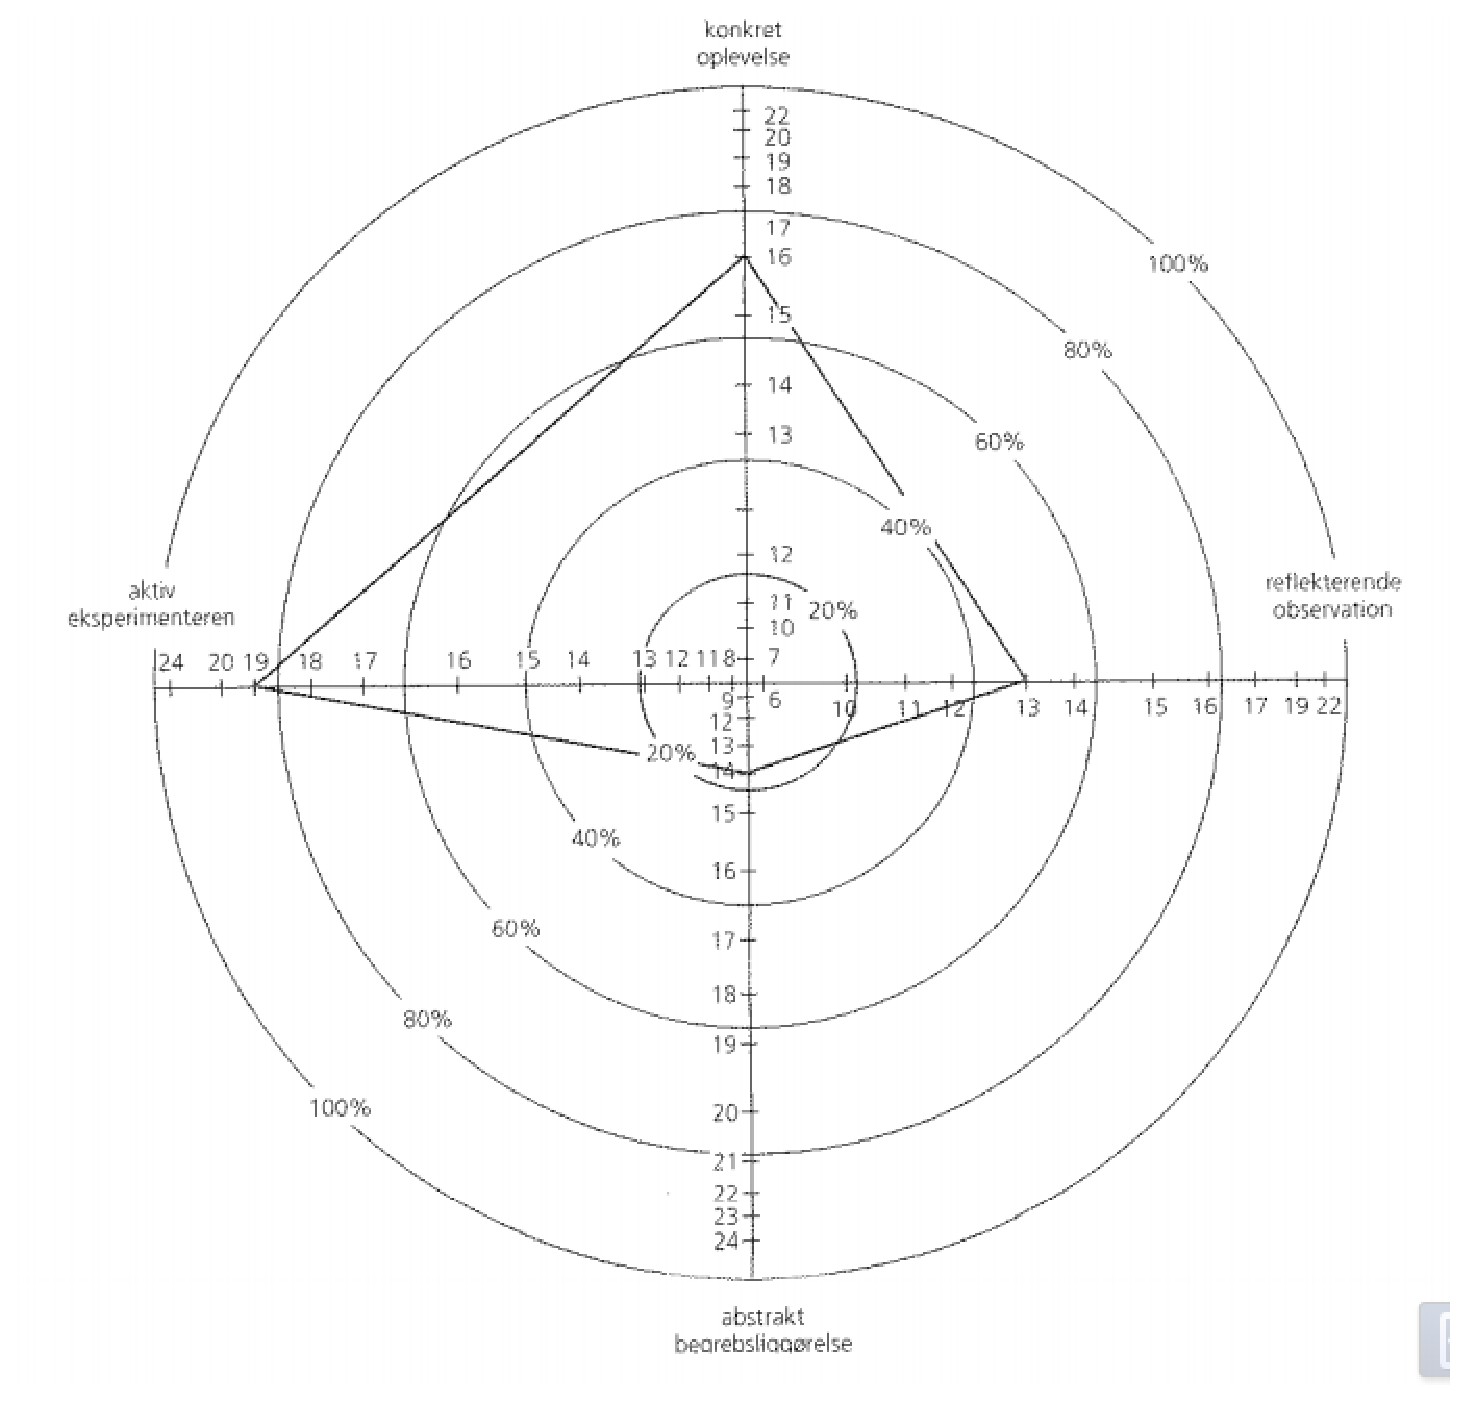
\includegraphics[width=6cm]{kolbstyle}
	\caption[M�ling af L�ringsstil]{Her vises resultatet af en l�ringsstils analyse af en socialarbejder, \citep{Illeris}}
	\label{fig:kolb2}
	\vspace{-5pt}
\end{wrapfigure}
Gennem dette forl�b var �nsket at arbejde med elev aktiverende undersvisning.  Udgangspunktet hvor eleven er i fokus l�gger automatisk op til at vi vil bev�ge os i retning af tanker som findes hos Dewey under mantraet ``Learning by doing'', men det er ikke blot gennem selv at arbejde med arbejdet at eleven opn�r en st�rre kognitiv forst�else af stoffet dette g�res ved at sende eleven p� en erfaringsbaseret rejse gennemstoffet. Hvorved vi g�r fra Deweys om end lidt firkantede tilgang til l�ring over og dykker ned i en mere forfinet teori som den udviklet af David Kolb. Kolbs l�ringsteorier er en udvidelse af Deweys teorier og kan beskrives som erfarringsbaseret l�ring, \citep{Illeris, Kolb:1984, Gympd}. I artiklen af \citep{Illeris} fremg�r det at vi skal passe p� med blot at anvende Kolbs l�ringsstile. 
Det fremg�r endvidere at Kolb testede sine teorier p� en r�kke af studerende i USA, her s� man et m�nster hvorefter de studerende fordeltes. Det viste sig at studerende p� fagene psykologi, polotogi og historie endte med ligge mellem den konkrete oplevelse og den reflekterende observation i \figref{kolb1}. Studerende p� fag som �konomi og sociologi havnede mellem den reflekterende observation og den abstrakte begrebsligg�relse, se igen \figref{kolb1}, studerende fra de naturvidenskablige fag fysik, kemi og matematik endte i kategorien abstrakt begrebsligg�relse. 

Ingeni�rer og Sygeplejersker ligger typisk mellem den abstrakt begrebsligg�relse og den aktive eksperimenteren p� \figref{kolb1} og sidst men ikke mindst havde vi studerende i handelssektoren som endte mellem den aktive eksperimenteren og den konkrete oplevelse. Derfor udviklede Kolb nogle erkendelses-niveauer i sin teori disse koblede de fire hovede omr�der, derved fik psykologi, polotogi og historie koblet den divergente erkendelse p�. �konomi og sociologi blev tilskrevet en assimilativ erkendelse. Ingeni�rer og sygeplejersker fik tilskrevet konvergent erkendelse og de naturvidenskabelige studerende l� imellem den assimilative erkendelse og den konvergente erkendelse dette blev til begribelse via forst�else. Sluttelig blev handelssektoren koblet med den akkomodative erkendelse, \citep{Illeris}.
Det skal dog hertil siges at det ikke er en ligefrem sag at bestemme en persons l�ringsstil. Af \figref{kolb2} fremg�r det at en l�ringsstil n�r den er bestemt kan illustreres som en polygon i en slags ``pol�rtkoordinatsystem''. Der findes flere tests som kan fastsl� en persons foretrukne l�ringsstil, jeg har f�et min egen testet gennem 4MAT\textregistered. Det er meget vigtigt for elevernes indl�ring af stoffet at man har stort kendskab til sin egen l�ringsstil og endvidere til andre typer af l�ringsstile, da dette er vigtigt for opn�elsen af god l�ring for eleverne.


%Opgavens tilgang til l�ring baseres i h�j grad p� det rationalisme, med baggrund i Kolbs l�rings teorier. Et af de tidligste mantraer inden for denne l�rings teori er ``\emph{Learning by doing}'' som stammer fra John Dewey 










\chapter{Opsamling og Konklusion}
\label{ch:konk}

Progression handler i daglig tale om at flytte sig, det kan v�re i form af ny viden som udvider ens egen horisont. Progression i faglighed handler i h�j grad om kompetencer og forst�else for hvis man ikke har forst�et den viden man har l�rt om kan man ikke anvende den, og kan man ikke anvende den forst�r man ikke dens kompleksitet. Som undervisere skal vi flytte eleverne fra et stadie hvor de m�ske er pr�-strukturelle til et niveau hvor de er relationelt t�nkende hvilket vil sige at de g�r fra et 0-niveau til et niveau hvor de kan forbinde og anvende begreber og centrale analyse metoder. Men f�r vi som undervisere kan flytte eleverne, skal de v�re villige til at l�re. Denne villighed fra elevernes side kan kun opst� hvis eleverne f�ler at de bliver taget seri�st og at de bliver udfordret p� deres eget niveau. Derfor er det vigtigt at man som underviser forst�r at optr�de i forskellige roller over for forskellige elever p� en gang, her kan man g�re brug af de fire l�ringsrum som Beck og Gottlieb pr�senterede i \citep{Beck:2002}, endvidere b�r man lede klassen jf. den situationsbestemte ledelse jf. \citep{Hersey1, Herse2}. N�r f�rst eleverne er inspirerede handler det om at give dem muligheder for at f� den personlige oplevelse og give dem det rum der g�r de kan reflektere over deres egen oplevelse derved skabe det fundament som Dewey beskriver giver anledning til l�ring.  Herved vil eleverne opn� ny viden og dermed ny indsigt som vil �bne faget for dem. Dette er kernen i den faglige progression. Den faglige progression opst�r alts� allerede i underviserens forberedelse af det enkelte forl�b, hvor underviseren g�r sig tanker om undervisningsformer, arbejdsstof, og hvor selve undervisningen tilrettel�gges. men ogs� empati og evnen til at fornemme hvor eleverne er er en naturlig del af det at skabe god progression for eleverne.

Gennem denne opgave har jeg s�gt at motivere at eleverne har et behov for ledelse omend ledelsen foreg�r i tilrettel�ggelsen af undervisningen \citep{EVA:2013, Meyer:2008, leder:2010, Alstrup:1997, DDS:2006, Hersey1, Herse2}.  Eller i selve afviklingen af en given aktivitet s� er det alfa omega at man som underviser hj�lper eleverne til at opn� den personlige oplevelse som kan starte en l�rings process om man s� er mere eller mindre styret af den l�replan man er underlagt s� er det altid underviserens ansvar at br�nde igennem til eleverne gennem sp�ndende og n�rv�rende undervisning.

Vi kan alts� konkludere at den faglige progression er et samspil mellem mange elementer, vi kan snakke om hvordan man i sin forberedelse sikre elevernes faglige progression denne kan v�re dikteret af l�replanen eller den kan v�re mere op til den enkelte underviser, I faget fysik er vi bundet af fagets l�replan, og faget har dermed en naturlig progression indbygget i den m�de kerne stoffet er struktureret p�. Det er dog �nskv�rdigt at indbygge yderligere progression i sine forl�b hvor vi gennem smarte valg af planl�gningsv�rkt�jer kan optimere vores process, og sikre progression for mange elevgrupper p� en gang. Her er v�rkt�jer som FIMME modellen, den didaktiske relationsmodel og 4MAT\textregistered ~de oplagte v�rkt�jer som vil g�re livet lettere for os som undervisere. Sluttelig er der selve afviklingen hvor vi som undervisere st�r p� m�l for den tilrettelagte progression i faget. Her skal vi hele tiden tilpasse planer og niveau efter forholdene og eleverne s�ledes at elverne f�r bygget det h�jest mulige korthus. Dermed er vi alts� ogs� n�dt til at hj�lpe forskellige elever p� forskellige m�der. Her er det efter min over bedste overbevisning vigtigt at have kendskab til personlighedstyper, jf. \citep{MBTI, JTI, DDS:2006, Alstrup:1997, Ringstad:2002} samt ledelse af forskellige individer p� forskellig m�de jf. \citep{Hersey1, Herse2, Alstrup:1997, DDS:2006}. Med andre ord;

\begin{quote}
	``\emph{Progression i undervisningen handler om m�lrettet ledelse.}''
\end{quote}\vspace{.75cm}

\begin{flushright}
Thomas Mellergaard Amby
\end{flushright}


\begin{appendix}
\chapter[Undervisnings forl�bet Verdensbilleder]{Verdensbilleder}
\label{app:Verden}
\section{~Form�l:}
Form�let med forl�bet om fysikkens bidrag til verdensbilleders udvikling, er at give eleverne en forst�else af at fysikken har bidraget til at udvikle dem m�de vi opfatter den verden vi lever i. Gennem eksperimenter og teoretiske betragtninger skal vi se p� hvorledes verden har �ndret sig fra Ptolemaios og frem til vore dages s�gen efter exoplaneter.

\section{~Indhold:}
Forl�bet vil v�re bygget op hhv. omkring stoffet i FysikABbogen 1�s kapitel 3 om verdensbilledet, men i liges� stor grad p� noter som vil blive udleveret i forbindelse med undervisningen. Disse noter vil v�re skrevet og tilrettelagt s�ledes at de bygger videre p� de kerne tekster som ligger i kapitlet fra Benoni et al. Forl�bet er t�nkt s� det f�lger en naturlig r�dtr�d gennem de �rstal som vi skal dykke ned i. Forl�bet t�nkes at l�be over 10 moduler af  90 min.

\section{~Metode:}
Metoden som t�nkes anvendt her, er hhv. eksperimentel da det er vigtigt for eleverne at l�re at s�tte ind i hvorledes man t�nkte i oldtiden, samt i ren�ssancen endda ogs� i nyere tid.  Gennem denne t�nkning vil eleverne ogs� indse hvorfor man har draget de slutninger man har. Andre typer af undervisningsformer som t�nkes anvendt er grupper og matrix grupper da fokus i klassen pt. Er p� elevaktiverende undervisning. Ydermere t�nkes der en teoretisk dimension, hvor vi snuser til meget af den underliggende teori, og i det store hele vil forl�bet tjene som en form or oversigts l�sning i hvilke interessante emner klassen skal igennem i det 2 �rige  B-niveau.

\section{~Materiale:}
Materialet vil som omtalt i afsnittet indhold prim�rt v�re kapitlet i bogen men ogs� noter fra timen vil blive anvendt som en del af undervisningens pensum, her t�nkes specielt p� opl�g til gruppe arbejde.

\section{~Evaluering:}
I forhold til evalueringen af dette forl�b t�nkes der at vi l�bende vil evaluere processen gennem sm� interaktive quizzer med programmet socrative (\href{http://m.socrative.com}{m.socrative.com}). Dette vil give os et direkte m�l for elevernes progression gennem forl�bet. Endvidere t�nkes det at eleverne skal skrive en rapport om nogle af de ting der er arbejdet med, for at give et helheds billeder af om eleverne har forst�et stoffet. 

\section{~Modul plan:}


\begin{table}
	\centering
	\caption[Verdensbilleder - Modul 1 -- Mit eget verdensbillede]{Modul 1 - Mit eget verdensbillede}
	\begin{tabular}{@{ } l p{2.5cm} p{4cm} p{5cm} @{ }}
		\toprule[2pt]
		{\bf Tid [min]} & {\bf Aktivitet} & {\bf Beskrivelse af aktivitet} & {\bf Didaktiske overvejelser}\\
		\midrule
		0 & Pr�sentation af dagens program & Kort skematisk pr�sentation af den film som skal ses & Dette g�res for at eleverne er bekendte med at der vil komme en opgave som forholder sig til filmen � og at der derfor kan v�re en ide at tage noter. \\
		\midrule
		3 & Se film & Vi ser filmen: Danskernes Akademi � Verdens st�rste fysikeksperiment  & At give eleverne en ny type indsigt i den verden de selv lever i.\\
		\midrule
		80 & Der samles op p� dagens afsnit af filmen & Vi n�r ikke at se hele filmen derfor samler vi kort op p� hvad vi har f�et at vide i dag, inden der rydes op og lokalet forlades & S�rg for at Eleverne tager noget med sig fra timen.\\
		\bottomrule[2pt]
	\end{tabular}
\end{table}


\begin{table}
	\centering
	\caption[Verdensbilleder - Modul 2 -- Mit eget verdensbillede del 2]{Modul 2 - Mit eget verdensbillede del 2}
	\begin{tabular}{@{ } l p{2.5cm} p{4cm} p{5cm} @{ }}
		\toprule[2pt]
		{\bf Tid [min]} & {\bf Aktivitet} & {\bf Beskrivelse af aktivitet} & {\bf Didaktiske overvejelser}\\
		\midrule
		0 & Pr�sentation af dagens program & Kort skematisk pr�sentation af den film som skal ses & Dette g�res for at eleverne er bekendte med at der vil komme en opgave som forholder sig til filmen � og at der derfor kan v�re en ide at tage noter. \\
		\midrule
		3 & Se film - fortsat & Vi ser filmen: Danskernes Akademi � Verdens st�rste fysikeksperiment  & At give eleverne en ny type indsigt i den verden de selv lever i.\\
		\midrule
		45 & Beskriv dit verdenssyn & Med udgangspunkt i filmen om CERN og LHC skal eleverne beskrive den verden de selv lever i og hvad konsekvensen for den almindelige dansker er. & Opgaven tvinger eleverne til at fundere over den verden de lever i og hvordan de opfatter den\\
		\midrule
		75 & Diskussion af verdensbilledet i dag plenum & Med udgangspkt. I en eller flere af elevernes beskrivelser af verdensbilledet i dag snakker vi om betydningen for den almene dansker & Diskussionen foreg�r i Plenum, men den forudg�ende skriftlige �velse sikre at alle har noget at byde ind med og at alle har gjort sig nogle overvejelser\\
		\midrule
		85 & Der ryddes op & Lokalet skal forlades p�nt og ordentligt & Tak for idag\ldots\\
		\bottomrule[2pt]
	\end{tabular}
\end{table}

\begin{table}
	\centering
	\caption[Verdensbilleder - Modul 3 -- Fra Aristoteles til Kopernikus]{Modul 3 - Fra Aristoteles til Kopernikus}
	\begin{tabular}{@{ } l p{2.5cm} p{4cm} p{5cm} @{ }}
		\toprule[2pt]
		{\bf Tid [min]} & {\bf Aktivitet} & {\bf Beskrivelse af aktivitet} & {\bf Didaktiske overvejelser}\\
		\midrule
		0 & Opsamling fra sidst & Kort opsummering af timen ig�r, Disse skal kort gennemg�es af eleverne p� tavlen. & Dette g�res for at sikre at alle har forst�et hvorledes verden i dag h�nger sammen\\
		\midrule
		10 & Pr�sentation af det nye emne � Mindmap p� tavlen. & Associativ �velse, �velsens form�l er at f� eleverne tili f�llesskab at finde ud af hvad et verdensbillede egentlig er og hvordan fysikken kan bidrage.  & Dette bliver totalt kaos, men vil give os en ide om elevernes forh�ndsforst�else for forl�bets indhold.\\
		\midrule
		30 & Pr�sentation af dagens n�gle personer. & Personerne som vi skal arbejde med skal pr�senteres  s�ledes at alle ved hvad hvem vi skal arbejde med og hvorledes de opfattede verden.  & At give eleverne et f�lles forforst�else for dagens arbejde i grupper.\\
		\midrule
		60 & Gruppe arbejde & Klassen deles i 6 grupper: tre grupper besk�ftiger sig med hvilke personer vi har i spil: Aristoteles, Ptolemaios og Kopernikus. 3 grupper laver eksperimenter, som man ville have gjort p� deres tid. Produktet skal v�re en 5 min. Pr�sentation for resten af klassen omhandlende resultater og/eller hvem personen var. &  Her gives resten af timen til fordybende arbejde. Med de tre kerne personer\\
		\midrule
		85 & Der rydes op & Lokalet skal forlades p�nt og ordenligt. & Hvordan var timens forl�b?
Feedback fra: Ahmed, Arina \& Casper Juul\\
		\bottomrule[2pt]
	\end{tabular}
\end{table}

\begin{table}
	\centering
	\caption[Verdensbilleder - Modul 4 -- Fra Kopernikus til Newton]{Modul 4 - Fra Kopernikus til Newton}
	\begin{tabular}{@{ } l p{2.5cm} p{4cm} p{5cm} @{ }}
		\toprule[2pt]
		{\bf Tid [min]} & {\bf Aktivitet} & {\bf Beskrivelse af aktivitet} & {\bf Didaktiske overvejelser}\\
		\midrule
		0 & Opsamling fra sidst & Vi gennemg�r de opgaver som grupperne havde sidst, hver gruppe m� max have 2 slides. & �velse I kort at pr�sentere udvalgt stof for en given m�lgruppe samt at vidensdele indternt (og p� FC)\\
		\midrule
		40 & Pr�sentation af dagens n�gle personer. & Personerne som vi skal arbejde med skal pr�senteres  s�ledes at alle ved hvad hvem vi skal arbejde med og hvorledes de opfattede verden. & Kernen her vil ligge i hvorledes verden s� ud inden Newton og hvilke landvindinger der var sket mellem antikken og s� frem til Gallilei. \\
		\midrule
		60 & Opl�g til par arbejde & Der give instrukser til hvorledes der skal arbejde resten af timen. & Dagens anden store elev aktivering vil ligge i form af et par arbejde. Her vil v�re nogle sp�rgsm�l som vil har deres udgangspunkt i den l�ste tekst. Samt nogle hvortil informations s�gning p� nettet vil v�re n�dvendig.\\
		\midrule
		85 & Der rydes op & Lokalet skal forlades p�nt og ordenligt.resultater og/eller hvem personen var. & Hvordan forl�b timen?
Feedback fra:
Casper O., Christian S. \& Gerd\\
		\bottomrule[2pt]
	\end{tabular}
\end{table}

\begin{table}
	\centering
	\caption[Verdensbilleder - Modul 5 -- Verden efter Newton]{Modul 5 - Verden efter Newton}
	\begin{tabular}{@{ } l p{2.5cm} p{4cm} p{5cm} @{ }}
		\toprule[2pt]
		{\bf Tid [min]} & {\bf Aktivitet} & {\bf Beskrivelse af aktivitet} & {\bf Didaktiske overvejelser}\\
		\midrule
		0 & Opsamling fra sidst & Vi gennemg�r det par arbejde som blev lavet sidst. & Her er �velsen at eleverne nu i lidt st�rrer grupper sammen gennemg�r det der blev lavet sidst.\\
		\midrule
		20 & Fra Newton til Hubble & Personerne som vi skal arbejde med skal pr�senteres  s�ledes at alle ved hvad hvem vi skal arbejde med og hvorledes de opfattede verden. & Kernen her vil ligge i hvorledes verden s� ud inden Newton og hvilke landvindinger der var sket mellem antikken og s� frem til Gallilei. \\
		\midrule
		60 & Gruppe arbejde om en r�kke opgaver. & Der regnes opgaver  & Hj�lpe med elevernes forst�else af stoffet.\\
		\midrule
		85 & Der rydes op & Lokalet skal forlades p�nt og ordenligt.resultater og/eller hvem personen var. & Hvordan forl�b timen?
Feedback fra:
Hamza, Hjalte \&Jakob\\
		\bottomrule[2pt]
	\end{tabular}
\end{table}

\begin{table}
	\centering
	\caption[Verdensbilleder - Modul 6 -- P� opdagelse i solsystemet]{Modul 6 - P� opdagelse i solsystemet}
	\begin{tabular}{@{ } l p{2.5cm} p{4cm} p{5cm} @{ }}
		\toprule[2pt]
		{\bf Tid [min]} & {\bf Aktivitet} & {\bf Beskrivelse af aktivitet} & {\bf Didaktiske overvejelser}\\
		\midrule
		0 & Opsamling fra sidst & Der samles kort op p� det arbejde som er blevet lavet frem til og med Hubble. Dermed �bner vi d�ren til astronomien & Plenums diskussion af hvordan verdensbilledet har udviklet sig siden Aristoteles. \\
		\midrule
		15 & Opl�g om solsystemets dannelse.  & Slide show gennemgang af solsystemets dannelse & H�j l�re styring for at sikre at alle har minimum en smal for-forst�else for dette emne inden gruppe arbejdet indledes\\
		\midrule
		45 & Del et af gruppe arbejde om solsystemet & Hver gruppe f�r en arbejdsseddel med sp�rgsm�l og ting som gruppen skal unders�ge. Ydermere skal gruppen give hinanden lektier for. & Opgaven er at eleverne selv fordyber sig i stoffet. Og bidrager til deres f�lles forst�else af stoffet\\
		\midrule
		85 & Der rydes op & Lokalet skal forlades p�nt og ordenligt.resultater og/eller hvem personen var. & Hvordan forl�b timen?
Feedback fra:
Jamie, Jeppe \& Jonas\\
		\bottomrule[2pt]
	\end{tabular}
\end{table}

\begin{table}
	\centering
	\caption[Verdensbilleder - Modul 7 -- P� opdagelse i solsystemet del 2]{Modul 7 - P� opdagelse i solsystemet del 2}
	\begin{tabular}{@{ } l p{2.5cm} p{4cm} p{5cm} @{ }}
		\toprule[2pt]
		{\bf Tid [min]} & {\bf Aktivitet} & {\bf Beskrivelse af aktivitet} & {\bf Didaktiske overvejelser}\\
		\midrule
		0 & 	Opsamling fra sidst & Grupperne fra sidst diskutere deres lektier s�ledes at de har en st�rre viden at tage med i matrix arbejdet. & �velsen her er at eleverne �ver sig i at formidle en specifik viden som kun de ligger inde med. (under tidspres)\\
		\midrule
		30 & MATRIX & Der formes nye grupper efter matrix princippet og der formidles nu med udgangspunkt i det som de indledende grupper havde haft som emne & Eleverne skulle nu opn� en mere generel forst�else af solsystemet og dets komponenter og spidsfindigheder.\\
		\midrule
		85 & Der rydes op & Lokalet skal forlades p�nt og ordenligt.resultater og/eller hvem personen var. & Hvordan forl�b timen?
Feedback fra:
Josephine, Kathrine\& Kristian\\
		\bottomrule[2pt]
	\end{tabular}
\end{table}

\begin{table}
	\centering
	\caption[Verdensbilleder - Modul 8 -- Jagten p� liv]{Modul 8 - Jagten p� liv}
	\begin{tabular}{@{ } l p{2.5cm} p{4cm} p{5cm} @{ }}
		\toprule[2pt]
		{\bf Tid [min]} & {\bf Aktivitet} & {\bf Beskrivelse af aktivitet} & {\bf Didaktiske overvejelser}\\
		\midrule
		0 & Opsamling fra sidst & Der samles op p� hvad vi har l�rt om solsystemet og de andre ting som har p�virket det verdensbillede vi har idag. & Dette g�res for at give eleverne overblik samt for at genopfriske detaljer.\\
		\midrule
		20 & Betydning af verdensbilledet  & Hvilken betydning har verdensbilledet for den forskning vi foretager i dag mhp. At finde liv andre steder end p� Jorden. & H�j l�rer styrring � pr�sentation af frontline data og forskning, med indlagte klasse diskussioner\\
		\midrule
		85 & Der rydes op & Lokalet skal forlades p�nt og ordenligt.resultater og/eller hvem personen var. & Hvordan forl�b timen?
Feedback fra:
Lasse, Louise \& Malale\\
		\bottomrule[2pt]
	\end{tabular}
\end{table}

\begin{table}
	\centering
	\caption[Verdensbilleder - Modul 9 -- Bestemmelse af Solens rotationstid]{Modul 9 - Bestemmelse af Solens rotationstid}
	\begin{tabular}{@{ } l p{2.5cm} p{4cm} p{5cm} @{ }}
		\toprule[2pt]
		{\bf Tid [min]} & {\bf Aktivitet} & {\bf Beskrivelse af aktivitet} & {\bf Didaktiske overvejelser}\\
		\midrule
		0 & Pr�sentation af fors�get & Her snakkes om hvorledes man kan gennemf�re eksperimentet. & Dette g�res for at give eleverne overblik samt for at genopfriske detaljer.\\
		\midrule
		10 & FORS�G  & Eleverne udf�rer eksperimentet p� data fra SOHO satellitten& Her f�r de en indsigt i at selv om man har den nyeste teknologi er der stadig nogle ting som man g�r p� en meget low-tech m�de.\\
		\midrule
		85 & Der rydes op & Lokalet skal forlades p�nt og ordenligt.resultater & Tak for idag\ldots\\
		\bottomrule[2pt]
	\end{tabular}
\end{table}

\begin{table}
	\centering
	\caption[Verdensbilleder - Modul 10 -- Bestemmelse af Solens rotationstid skrivemodul]{Modul 10 - Bestemmelse af Solens rotationstid skrivemodul}
	\begin{tabular}{@{ } l p{2.5cm} p{4cm} p{5cm} @{ }}
		\toprule[2pt]
		{\bf Tid [min]} & {\bf Aktivitet} & {\bf Beskrivelse af aktivitet} & {\bf Didaktiske overvejelser}\\
		\midrule
		0 & Opsamling p� fors�get & Vi diskuterer resultater og metoder & Gennemvejledning skulle slutproduktet gerne v�re af h�jere kvalitet\\
		\midrule
		10 & Skrive tid  & Eleverne f�r modulet til at skrive rapport i og stille sp�rgsm�l hvis de er i tvivl. & Her f�r de en indsigt i at selv om man har den nyeste teknologi er der stadig nogle ting som man g�r p� en meget low-tech m�de.\\
		\midrule
		85 & Der rydes op & Lokalet skal forlades p�nt og ordenligt.resultater & Tak for idag\ldots\\
		\bottomrule[2pt]
	\end{tabular}
\end{table}


\end{appendix}

\backmatter
%\begin{thebibliography}{}
\bibliography{bibliografi/bibliografi}
%\end{thebibliography}

\end{document}